\afterpage{
  \begin{landscape}
    \chapter{\ifenglish Sensor's schematic\else แบบวงจรของอุปกรณ์วัด\fi}
    \begin{figure}[h!]
        \begin{center}
          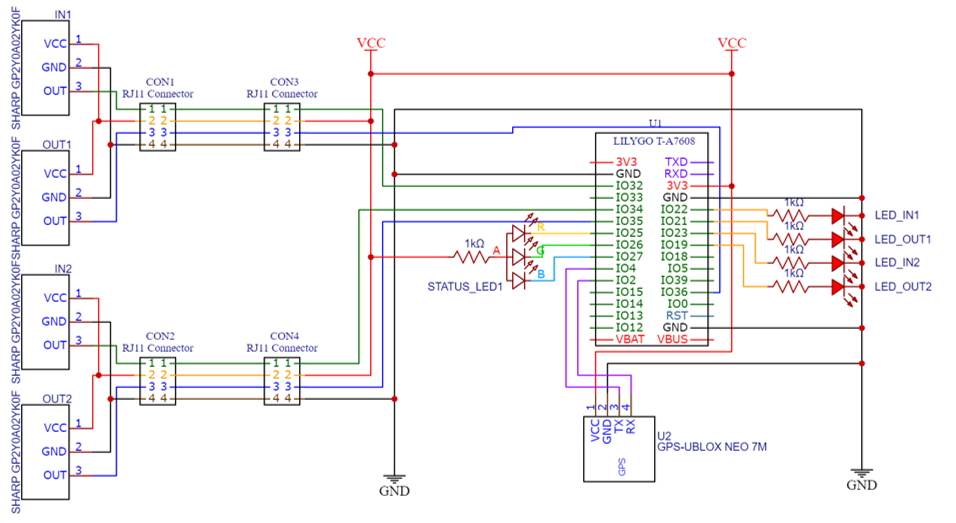
\includegraphics[width=\textwidth]{schematic.png}
        \end{center}
        \caption{เแบบวงจรของอุปกรณ์วัด}
        \label{fig:schematic}
      \end{figure}
  \end{landscape}
  }

\afterpage{
  \begin{landscape}
    \chapter{\ifenglish Sensor's State Machine\else State Machine ของอุปกรณ์วัด\fi}
    \begin{figure}[h!]
        \begin{center}
          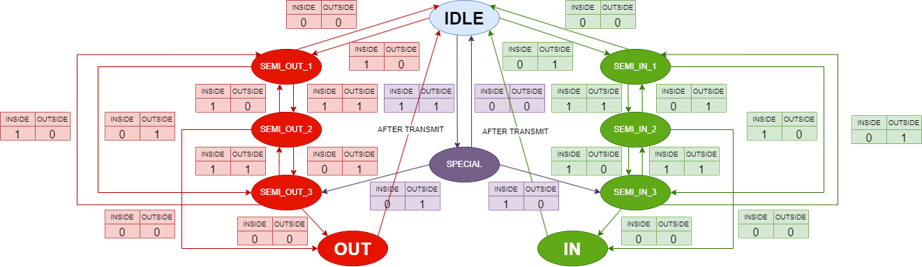
\includegraphics[width=\textwidth]{state-machine.png}
        \end{center}
        \caption{เแบบวงจรของอุปกรณ์วัด}
        \label{fig:state-machine-l}
    \end{figure}
  \end{landscape}
  }

\chapter{\ifenglish Test equipment installation\else การติดตั้งอุปกรณ์ทดสอบ\fi}
\section{ส่วนประมวลผล}
    \begin{figure}[h!]
        \begin{center}
        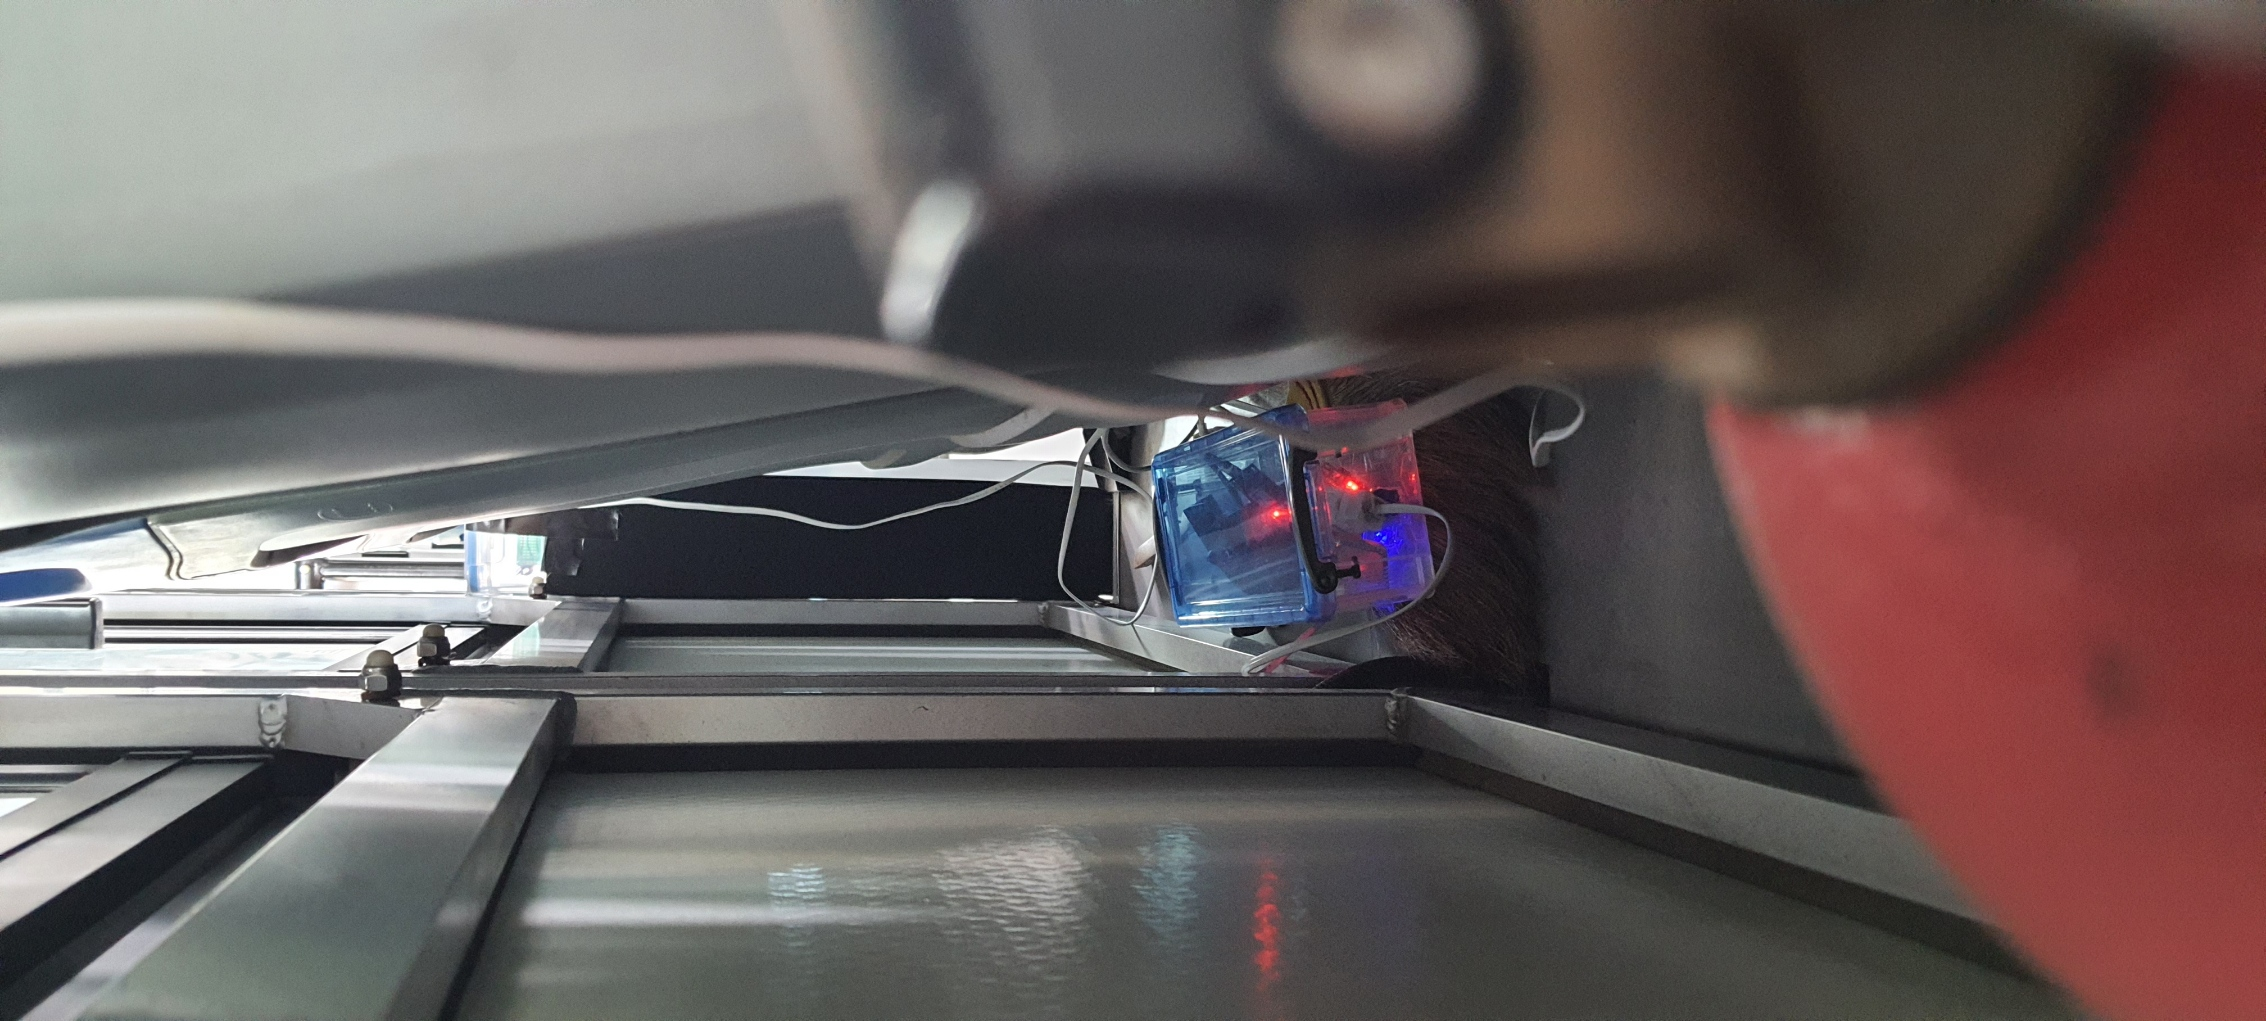
\includegraphics[width=\textwidth,angle=-90,origin=c]{install_mid.jpg}
        \end{center}
        \caption{การติดตั้งส่วนประมวลผล}
        \label{fig:install_mid}
    \end{figure}
    ติดตั้งส่วนประมวลผลที่เบาะหลังระหว่างประตูของรถโดยสาร
\pagebreak
\section{ส่วนอุปกรณ์วัดประตูผู้โดยสารกลาง}
    \begin{figure}[h!]
        \begin{center}
        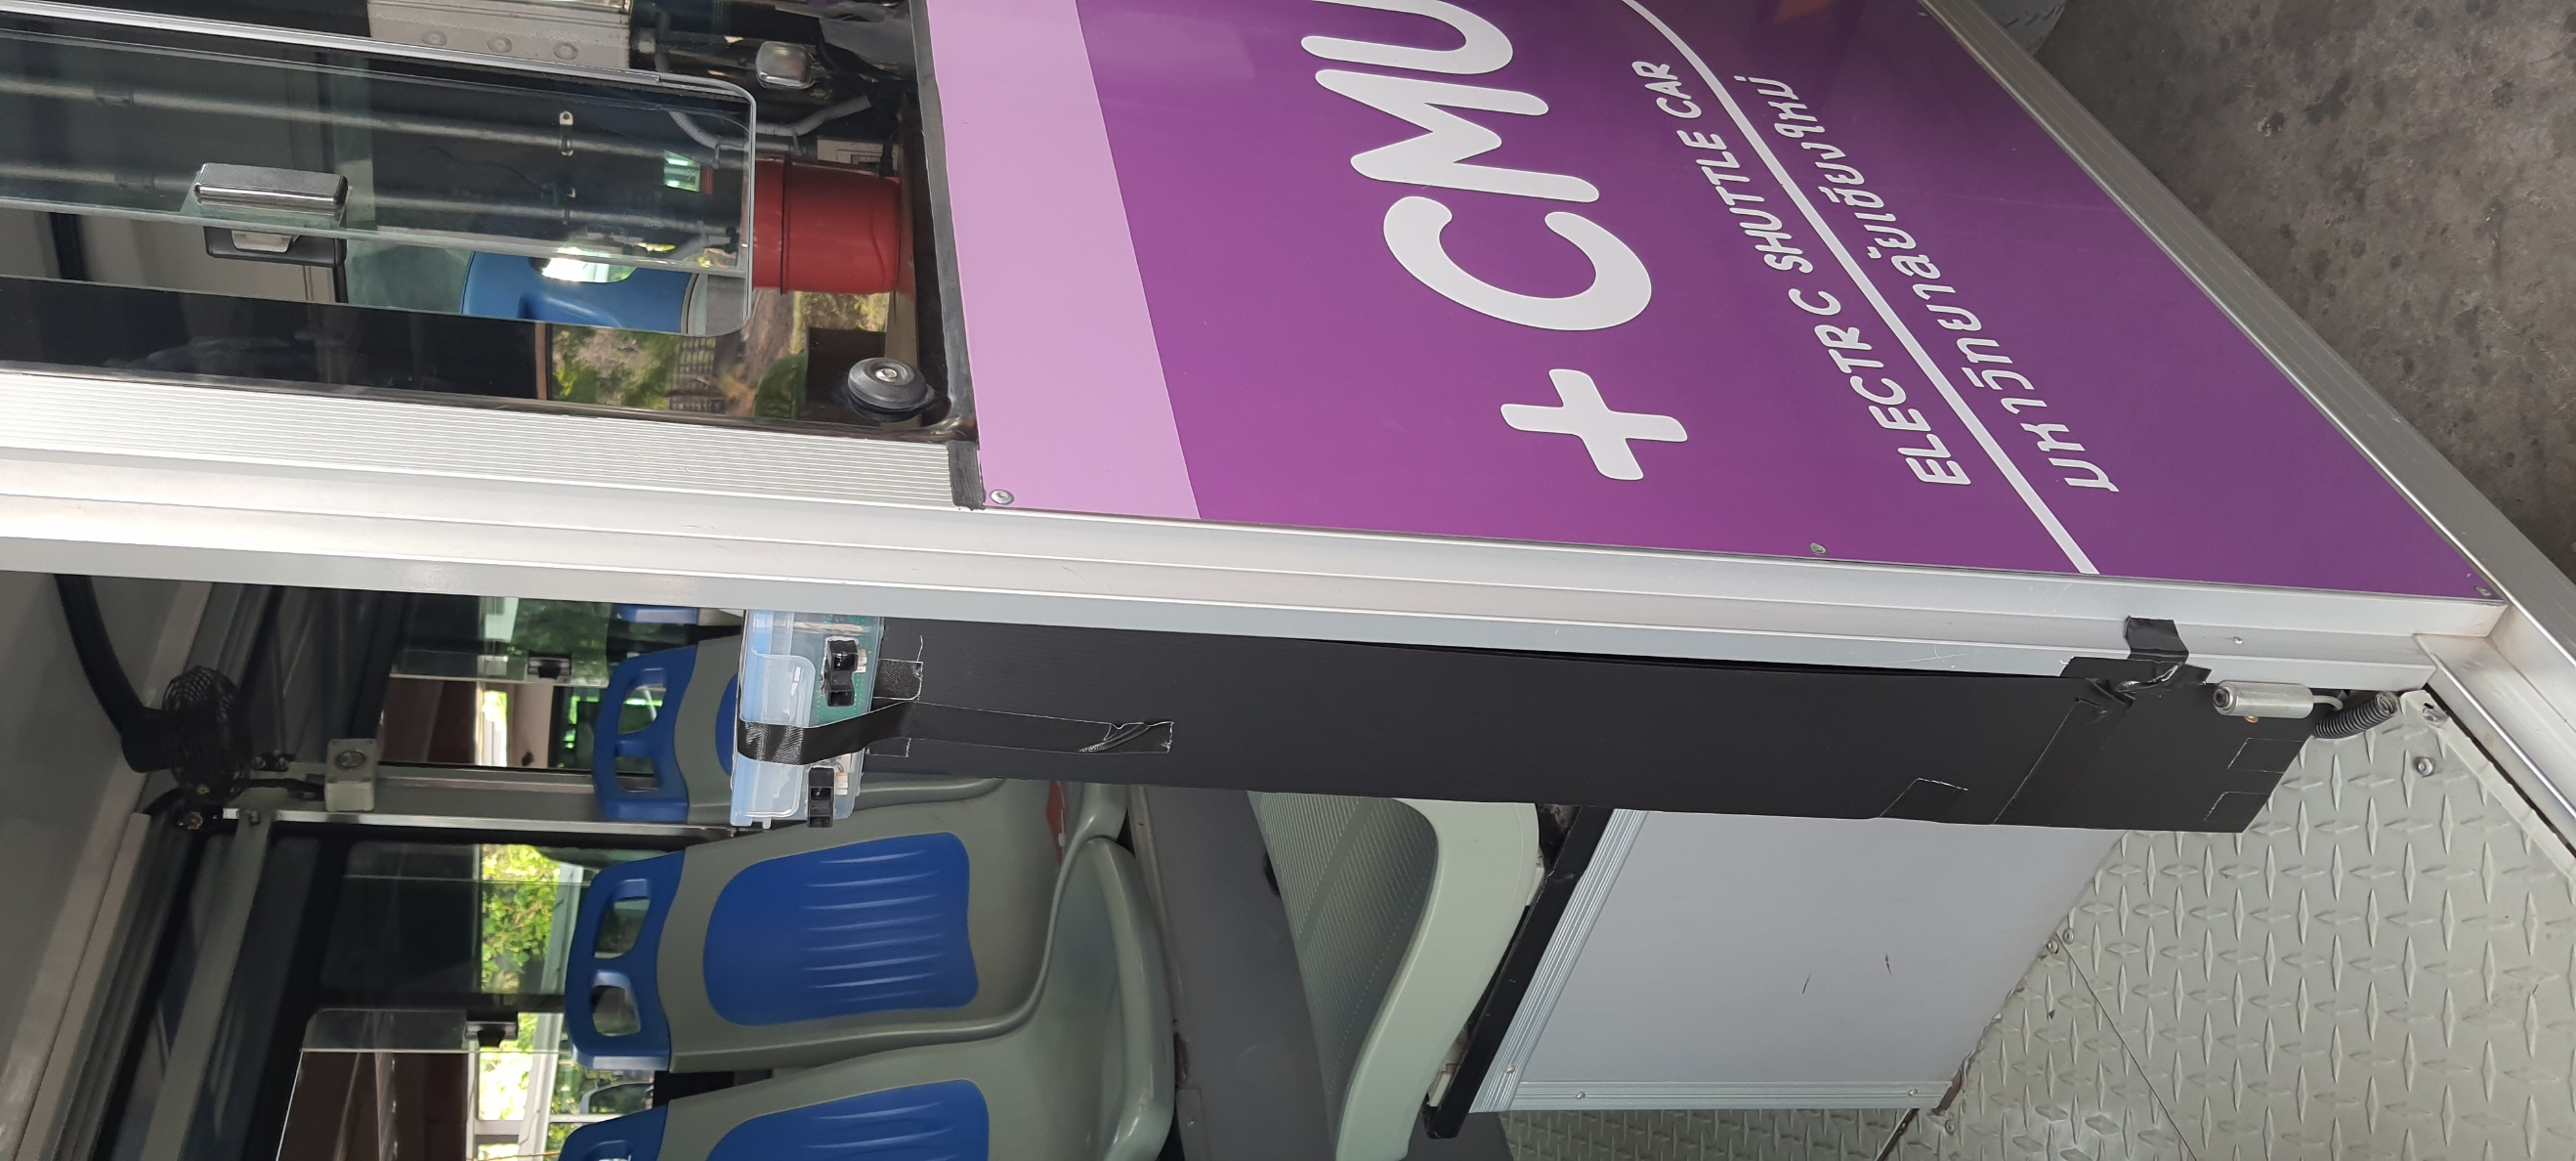
\includegraphics[width=\textwidth,angle=-90,origin=c]{install_front.jpg}
        \end{center}
        \caption{การติดตั้งส่วนอุปกรณ์วัดประตูผู้โดยสารกลาง}
        \label{fig:install_front}
    \end{figure}
    ติดสูงเหนือจากพื้น 80 เซนติเมตร
\pagebreak
\section{ส่วนอุปกรณ์วัดประตูผู้โดยสารหลัง}
    \begin{figure}[h!]
        \begin{center}
        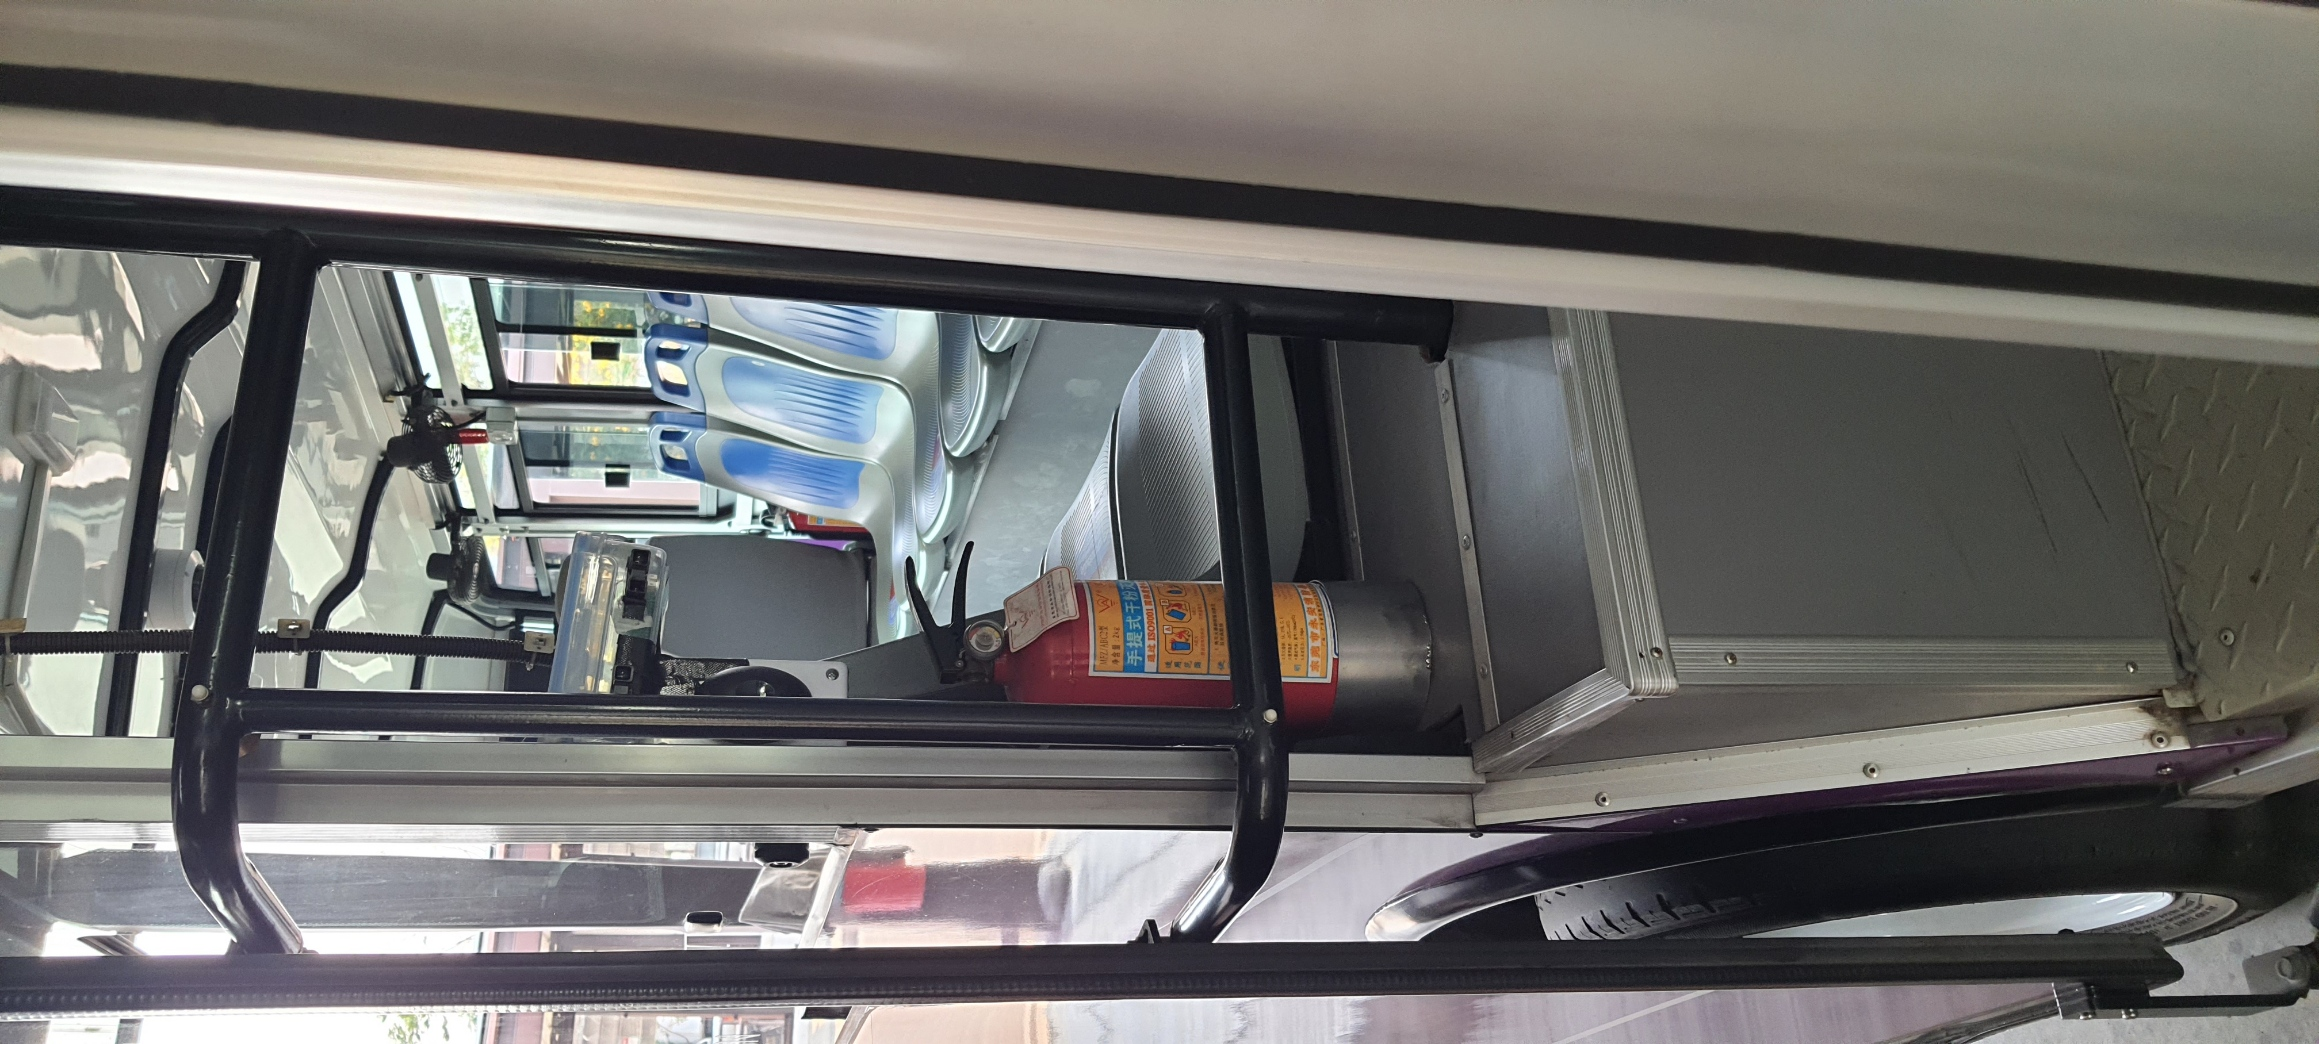
\includegraphics[width=\textwidth,angle=-90,origin=c]{install_back.jpg}
        \end{center}
        \caption{การติดตั้งส่วนอุปกรณ์วัดประตูผู้โดยสารหลัง}
        \label{fig:install_back}
    \end{figure}
    ติดสูงเหนือจากพื้น 75 เซนติเมตร

โดยส่วนอุปกรณ์วัดจะเชื่อมต่อกับส่วนประมวลผลด้วยสาย RJ11

\chapter{\ifenglish Manual\else คู่มือการใช้งานระบบ\fi}

\section{การติดตั้งโปรแกรมบนอุปกรณ์วัด}
    หลังจากต่อวงจรตามแบบวงจรและใส่ซิมการ์ดที่มีอินเตอร์เน็ตแล้ว ทำการ git clone ที่ \url{https://github.com/IkaWaAyuMu/261492-hw} เปิดผ่าน Visual Studio Code ที่ลง platform.io ไว้ จากนั้นตั้งค่า src/MQTT\_credentials.h.sample ให้เรียบร้อยแล้วเแลี่ยนชื่อเป็น src/MQTT\_credentials.h และทำการอัพโหลดโปรแกรมลงในอุปกรณ์วัด หากต้องการตั้งค่าใดๆ เช่น pin สามารถตั้งได้ที่ src/utilities.h

\section{การติดตั้งเซิฟเวอร์}
    ทำการ git clone ที่ \url{https://github.com/DifficultIV/261492-Backend} จากนั้นให้ทำการพิมพ์คำสั่ง npm install ลงใน terminal เพื่อทำการโหลดข้อมูลที่ต้องใช้(ใช้คำสั่งนี้เพียงครั้งแรกเท่านั้น) และพิมพ์คำสั่ง node --env-file=.env server.js เพื่อทำการเริ่มการทำงานของเซิฟเวอร์

\section{การติดตั้งเว็บไซต์}    
    ทำการ git clone ที่ \url{https://github.com/DifficultIV/261492-Occupancy-monitoring} จากนั้นให้ทำการพิมพ์คำสั่ง cd react-app ลงใน terminal เพื่อเข้าไปยังโฟลเดอร์ react-app จากนั้นให้ทำการพิมพ์คำสั่ง npm install เพื่อทำการโหลดข้อมูลที่ต้องใช้(ใช้คำสั่งนี้เพียงครั้งแรกเท่านั้น) และพิมพ์คำสั่ง npm start เพื่อทำการเริ่มการทำงานของเว็บไซต์